\documentclass{scrartcl}
\usepackage[T1]{fontenc}

% u/ masukin gambar
\usepackage{graphicx}

% u/ bikin ornament

% u/ mengatur margin kertas
\usepackage{geometry}
\geometry{
	a4paper,
	left=3.5cm,
	right=2.5cm,
	bottom=2.5cm,
	top=3cm
}

% u/ referensi
\usepackage{hyperref}

% u/ bikin tabel
\usepackage{tabu}
\usepackage{booktabs}

% u/ masukin source code
\usepackage{minted}
\usemintedstyle{vs}
\setminted[]{
	breaklines=true,
	tabsize=2,
	autogobble=true
}

% Content -> Daftar Isi
\renewcommand{\contentsname}{Daftar Isi}

\begin{document}
	
	% kop judul handout
	\begin{center}
		\begin{tabu} to \linewidth {X[c]}
			\toprule
			\\
			\LARGE{\textbf{Handout Praktikum Mobile Application}} \\
			\\
			\large{Topik 1 -- Activity dan Intent} \\
			\\
			\bottomrule
		\end{tabu}
	\end{center}
	
	\tableofcontents
	
	\section{Tujuan}
	
	\begin{enumerate}
		\item Mahasiswa dapat mengetahui cara menyimpan data sederhana menggunakan obyek \texttt{SharedPreferences}
		\item Mahasiswa dapat mengetahui cara memperbolehkan pengguna untuk memodifikasi preferensi menggunakan kelas \texttt{PreferenceActivity}
		\item Mahasiswa dapat mengetahui cara menulis dan membaca file dari penyimpanan internal dan eksternal
		\item Mahasiswa dapat mengetahui cara membuat dan menggunakan basis data SQLite
	\end{enumerate}
	
	\section{Komponen/Peralatan}
	
	\begin{itemize}
		\item PC/laptop
		\item Android Studio
	\end{itemize}
	
	\section{Dasar Teori}
	
	\section{Langkah Praktikum}
	
	\subsection{Menyimpan Data Menggunakan Obyek \texttt{SharedPreferences}}
	
	\begin{enumerate}
		\item Buat proyek baru dengan nama \textbf{UsingPreferences} (opsi yang lain dibiarkan \textit{default}).
		
		\item Buat file baru dengan nama \texttt{myapppreferences.xml}, lalu taruh di direktori \\ \texttt{app/res/xml/}.
		
		\item Buka \texttt{myapppreferences.xml}, lalu \textit{copy-paste} listing di bawah ini.
		
		\begin{minted}{xml}
		<?xml version="1.0" encoding="utf-8"?>
		<PreferenceScreen
			xmlns:android="http://schemas.android.com/apk/res/android">
			<PreferenceCategory android:title="Category 1">
				<CheckBoxPreference
					android:title="Checkbox"
					android:defaultValue="false"
					android:summary="True or False"
					android:key="checkboxPref" />
			</PreferenceCategory>
			<PreferenceCategory android:title="Category 2">
				<EditTextPreference
					android:hint="[Enter a string here]"
					android:summary="Enter a string"
					android:title="Edit Text"
					android:key="editTextPref" />
				<RingtonePreference
					android:summary="Select a ringtone"
					android:title="Ringtones"
					android:key="ringtonePref" />
				<PreferenceScreen
					android:title="Second Preference Screen"
					android:summary=
					"Click here to go to the second Preference Screen"
					android:key="secondPrefScreenPref" >
					<EditTextPreference
					android:hint="[Enter a string here]"
					android:summary="Enter a string"
					android:title="Edit Text (second Screen)"
					android:key="secondEditTextPref" />
				</PreferenceScreen>
			</PreferenceCategory>
		</PreferenceScreen>
		\end{minted}
		
		\item Buat file baru dengan nama \texttt{prefheaders.xml}, lalu taruh di direktori \texttt{app/res/xml/}
		
		\item Buka \texttt{prefheaders.xml} lalu \textit{copy-paste} listing berikut ini.
		
		\begin{minted}{xml}
		<?xml version="1.0" encoding="utf-8"?>
		<preference-headers
			xmlns:android="http://schemas.android.com/apk/res/android">
			<header android:fragment= 
				"com.example.usingpreferences.AppPreferenceActivity$PrefFragment"
				android:title="Preferences"
				android:summary="Sample preferences" />
		</preference-headers>
		\end{minted}
		
		\item Buat file baru dengan nama \texttt{AppPreferenceActivity.java}, lalu taruh di direktori \texttt{app/java/com.example.usingpreferences}
		
		\item Buka file \texttt{AppPreferenceActivity.java}, lalu \textit{copy-paste} listing berikut ini.
		
		\begin{minted}{java}
		package com.example.usingpreferences;
		
		import android.os.Bundle;
		import android.preference.PreferenceActivity;
		import android.preference.PreferenceFragment;
		import android.preference.PreferenceManager;
		
		import java.util.List;
		
		public class AppPreferenceActivity extends PreferenceActivity {
		
			@Override
			public void onCreate(Bundle savedInstanceState) {
				super.onCreate(savedInstanceState);
			}
			
			@Override
			public void onBuildHeaders(List<Header> target) {
				loadHeadersFromResource(R.xml.prefheaders, target);
			}
			
			@Override
				protected boolean isValidFragment(String fragmentName) {
				return true;
			}
			
			public static class PrefFragment extends   PreferenceFragment {
				@Override
				public void onCreate(Bundle savedInstanceState) {
					super.onCreate(savedInstanceState);
			
					PreferenceManager.setDefaultValues(getActivity(),
					R.xml.myapppreferences, false);
			
					// load the preferences from an XML resource
					addPreferencesFromResource(R.xml.myapppreferences);
				}
			}
		}
		\end{minted}
		
		\item Buka \texttt{AndroidManifest.xml}, lalu \textit{copy-paste} listing berikut ini.
		
		\begin{minted}{xml}
		<?xml version="1.0" encoding="utf-8"?>
		<manifest xmlns:android="http://schemas.android.com/apk/res/android"
			package="com.example.usingpreferences">
			
			<application
				android:allowBackup="true"
				android:icon="@mipmap/ic_launcher"
				android:label="@string/app_name"
				android:roundIcon="@mipmap/ic_launcher_round"
				android:supportsRtl="true"
				android:theme="@style/AppTheme">
				<activity android:name=".MainActivity">
					<intent-filter>
						<action android:name="android.intent.action.MAIN" />
						<category android:name="android.intent.category.LAUNCHER" />
					</intent-filter>
				</activity>
				<activity
					android:name=".AppPreferenceActivity"
					android:label="@string/app_name" >
					<intent-filter>
						<action android:name="com.example.AppPreferenceActivity" />
						<category android:name="android.intent.category.DEFAULT" />
					</intent-filter>
				</activity>
			</application>
		
		</manifest>
		\end{minted}
		
		\item Buka \texttt{activity\_main.xml}, lalu \textit{copy-paste} listing berikut ini.
		
		\begin{minted}{xml}
		<?xml version="1.0" encoding="utf-8"?>
		<android.support.constraint.ConstraintLayout xmlns:android="http://schemas.android.com/apk/res/android"
			xmlns:app="http://schemas.android.com/apk/res-auto"
			xmlns:tools="http://schemas.android.com/tools"
			android:id="@+id/activity_main"
			android:layout_width="match_parent"
			android:layout_height="match_parent"
			tools:context="com.example.usingpreferences.MainActivity">
			
			<Button
				android:text="Load Preferences Screen"
				android:layout_width="310dp"
				android:layout_height="wrap_content"
				android:id="@+id/btnPreferences"
				app:layout_constraintLeft_toLeftOf="@+id/activity_main"
				android:layout_marginStart="40dp"
				app:layout_constraintTop_toTopOf="@+id/activity_main"
				android:layout_marginTop="16dp"
				app:layout_constraintRight_toRightOf="@+id/activity_main"
				android:layout_marginEnd="16dp"
				app:layout_constraintBottom_toBottomOf="@+id/activity_main"
				android:layout_marginBottom="16dp"
				app:layout_constraintVertical_bias="0.0"
				android:onClick="onClickLoad"
				android:layout_marginRight="16dp"
				android:layout_marginLeft="40dp" />
			<Button
				android:text="Display Preferences Values"
				android:layout_width="310dp"
				android:layout_height="wrap_content"
				android:id="@+id/btnDisplayValues"
				app:layout_constraintLeft_toLeftOf="@+id/btnPreferences"
				app:layout_constraintTop_toBottomOf="@+id/btnPreferences"
				android:layout_marginTop="16dp"
				app:layout_constraintRight_toRightOf="@+id/btnPreferences"
				android:onClick="onClickDisplay"/>
			<EditText
				android:layout_width="310dp"
				android:layout_height="wrap_content"
				android:inputType="textPersonName"
				android:ems="10"
				android:id="@+id/editText"
				app:layout_constraintLeft_toLeftOf="@+id/btnPreferences"
				app:layout_constraintTop_toBottomOf="@+id/btnDisplayValues"
				android:layout_marginTop="16dp"
				app:layout_constraintRight_toRightOf="@+id/btnPreferences" />
			<Button
				android:text="Modify Preferences Values"
				android:layout_width="fill_parent"
				android:layout_height="wrap_content"
				android:id="@+id/btnModifyValues"
				app:layout_constraintLeft_toLeftOf="@+id/btnDisplayValues"
				app:layout_constraintTop_toBottomOf="@+id/editText"
				android:layout_marginTop="16dp"
				app:layout_constraintRight_toRightOf="@+id/btnDisplayValues"
				android:onClick="onClickModify" />
		
		</android.support.constraint.ConstraintLayout>
		\end{minted}
		
		\item Buka \texttt{MainActivity.java}, lalu \textit{copy-paste} listing berikut ini.
		
		\begin{minted}{java}
		package com.example.usingpreferences;
		
		import android.content.Intent;
		import android.os.Bundle;
		import android.support.v7.app.AppCompatActivity;
		import android.view.View;
		
		public class MainActivity extends AppCompatActivity {
		
			@Override
			protected void onCreate(Bundle savedInstanceState) {
				super.onCreate(savedInstanceState);
				setContentView(R.layout.activity_main);
			}
			
			public void onClickDisplay(View view) {
			}
			
			public void onClickModify(View view) {
			}
			
			public void onClickLoad(View view) {
				Intent i = new Intent("com.example.AppPreferenceActivity");
				startActivity(i);
			}
		}
		
		\end{minted}
		
		\item Tekan \texttt{Shift + F9} (atau pilih \texttt{Run > Debug}) untuk men-\textit{debug} aplikasi. Pilih salah satu Android Virtual Device yang kalian inginkan. Hasil akhir ditunjukkan pada Figur \ref{fig:screenshot001}.
		
			\begin{figure}[htbp]
			\begin{minipage}{.5\textwidth}
				\centering
				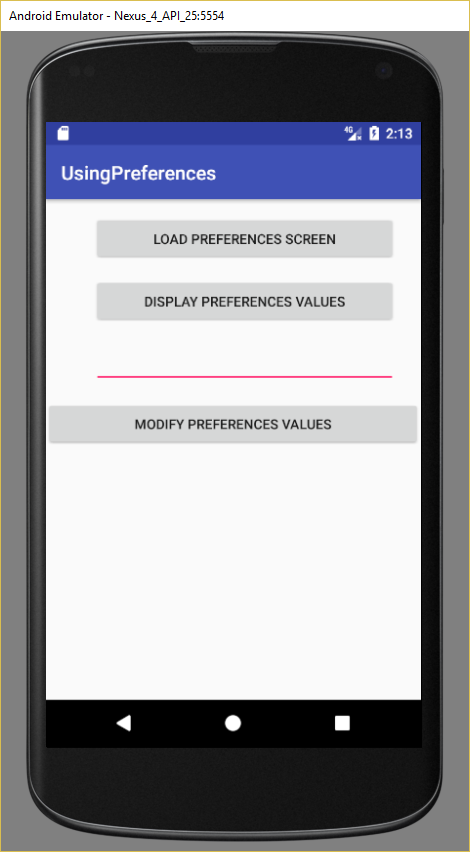
\includegraphics[width=0.7\linewidth]{screenshot001}
				\caption{Hasil Akhir (1)}
				\label{fig:screenshot001}
			\end{minipage}
			\begin{minipage}{.5\textwidth}
				\centering
				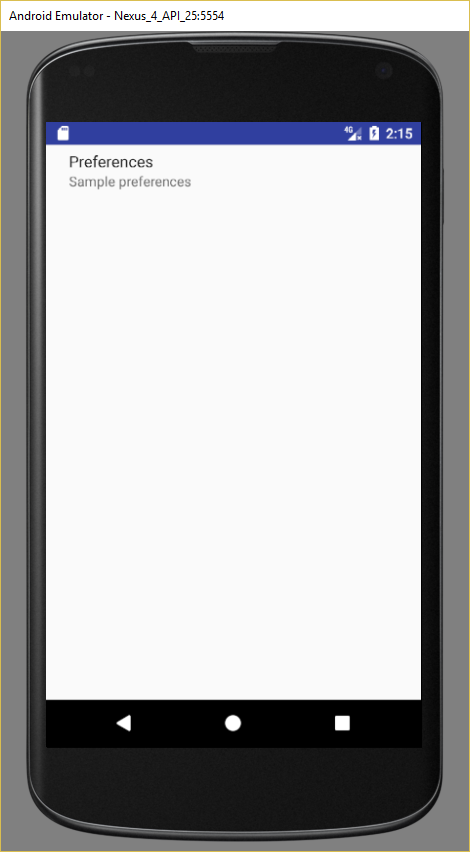
\includegraphics[width=0.7\linewidth]{screenshot002}
				\caption{}
				\label{fig:screenshot002}
			\end{minipage}
		\end{figure}
		
		\item Pilih \texttt{LOAD PREFERENCES SCREEN} untuk melihat layar Preference Header. Hasil akhir ditunjukkan pada Figur \ref{fig:screenshot002}
		
		\item Pilih \texttt{Preferences} untuk melihat layar Preferences.
		
	\end{enumerate}
	

\end{document}